\section{Richard-Germay-Detournay Family of Bit Model}
%\section{RGD Family of Models}
\label{ch:rgdmodels}

\subsection{Introduction}
While the current project focuses on drill string models, it is natural to couple a string model with a bit model. The Richard-Germay-Detournay family of bit models (RGD models) represents theoretical bit-rock interactions. They use a more sophisticated approach than many bit models and are, therefore, of interest. The RGD model is developed by Richard et al., 2007\ \cite{ref:richard2007a}, which simulates coupled axial and torsional vibration mode through bit-rock interaction. The model is widely applied to numerous drill-string models by providing sophisticated bit-rock interactions.
\subsection{RGD Model}
The model combines governing equations of motions (axial and torsional) with bit-rock interface law which leads to state-dependent delay system. Also the model takes in to account the loss of contact at wearflat/rock interface caused by axial vibration of the bit through discontinuous boundary conditions. Brief decription of mathematical background is shown in \figurename~\ref{figure_RGD_Summary}. The torsional and axial mode are coupled by bit-rock interaction model by the depth of cut. Moreover, functions $T_c$, $T_f$, $W_C$, and $W_f$ are defined with respect to drilling regime which reflects the discontinous boundary conditions. The drilling regimes are classified as following 1) cutting ($\omega>0, d>0$), 2) sticking ($\omega=0, d>0$) 3) sliding ($\omega>0, d=0$), 4) and off-bottom ($\omega>0, d<0$). The system is characterized to two degrees of freedom system with neglected any damping by assuming most of the energy dissipation in drilling systems is occuring at the bit-rock interface. The base assumptions of the model are: 1) constant angular velocity and upward force at the top of the drill string (fixed boundary conditions), 2) Vertical borehole, and 3) No lateral motions of the bit. The self-excited vibration was demonstrated and the model was also validated with laboratory tests. However, since the model is a bit model (not a drill string model), and limited to vertical well, it was not selected for this project. Moreover, because of the limited degrees of freedom, the model was not able to capture stick-slip occurence at frequency higher than first torsional mode. 

\begin{figure}[!hbt]
  \centering
  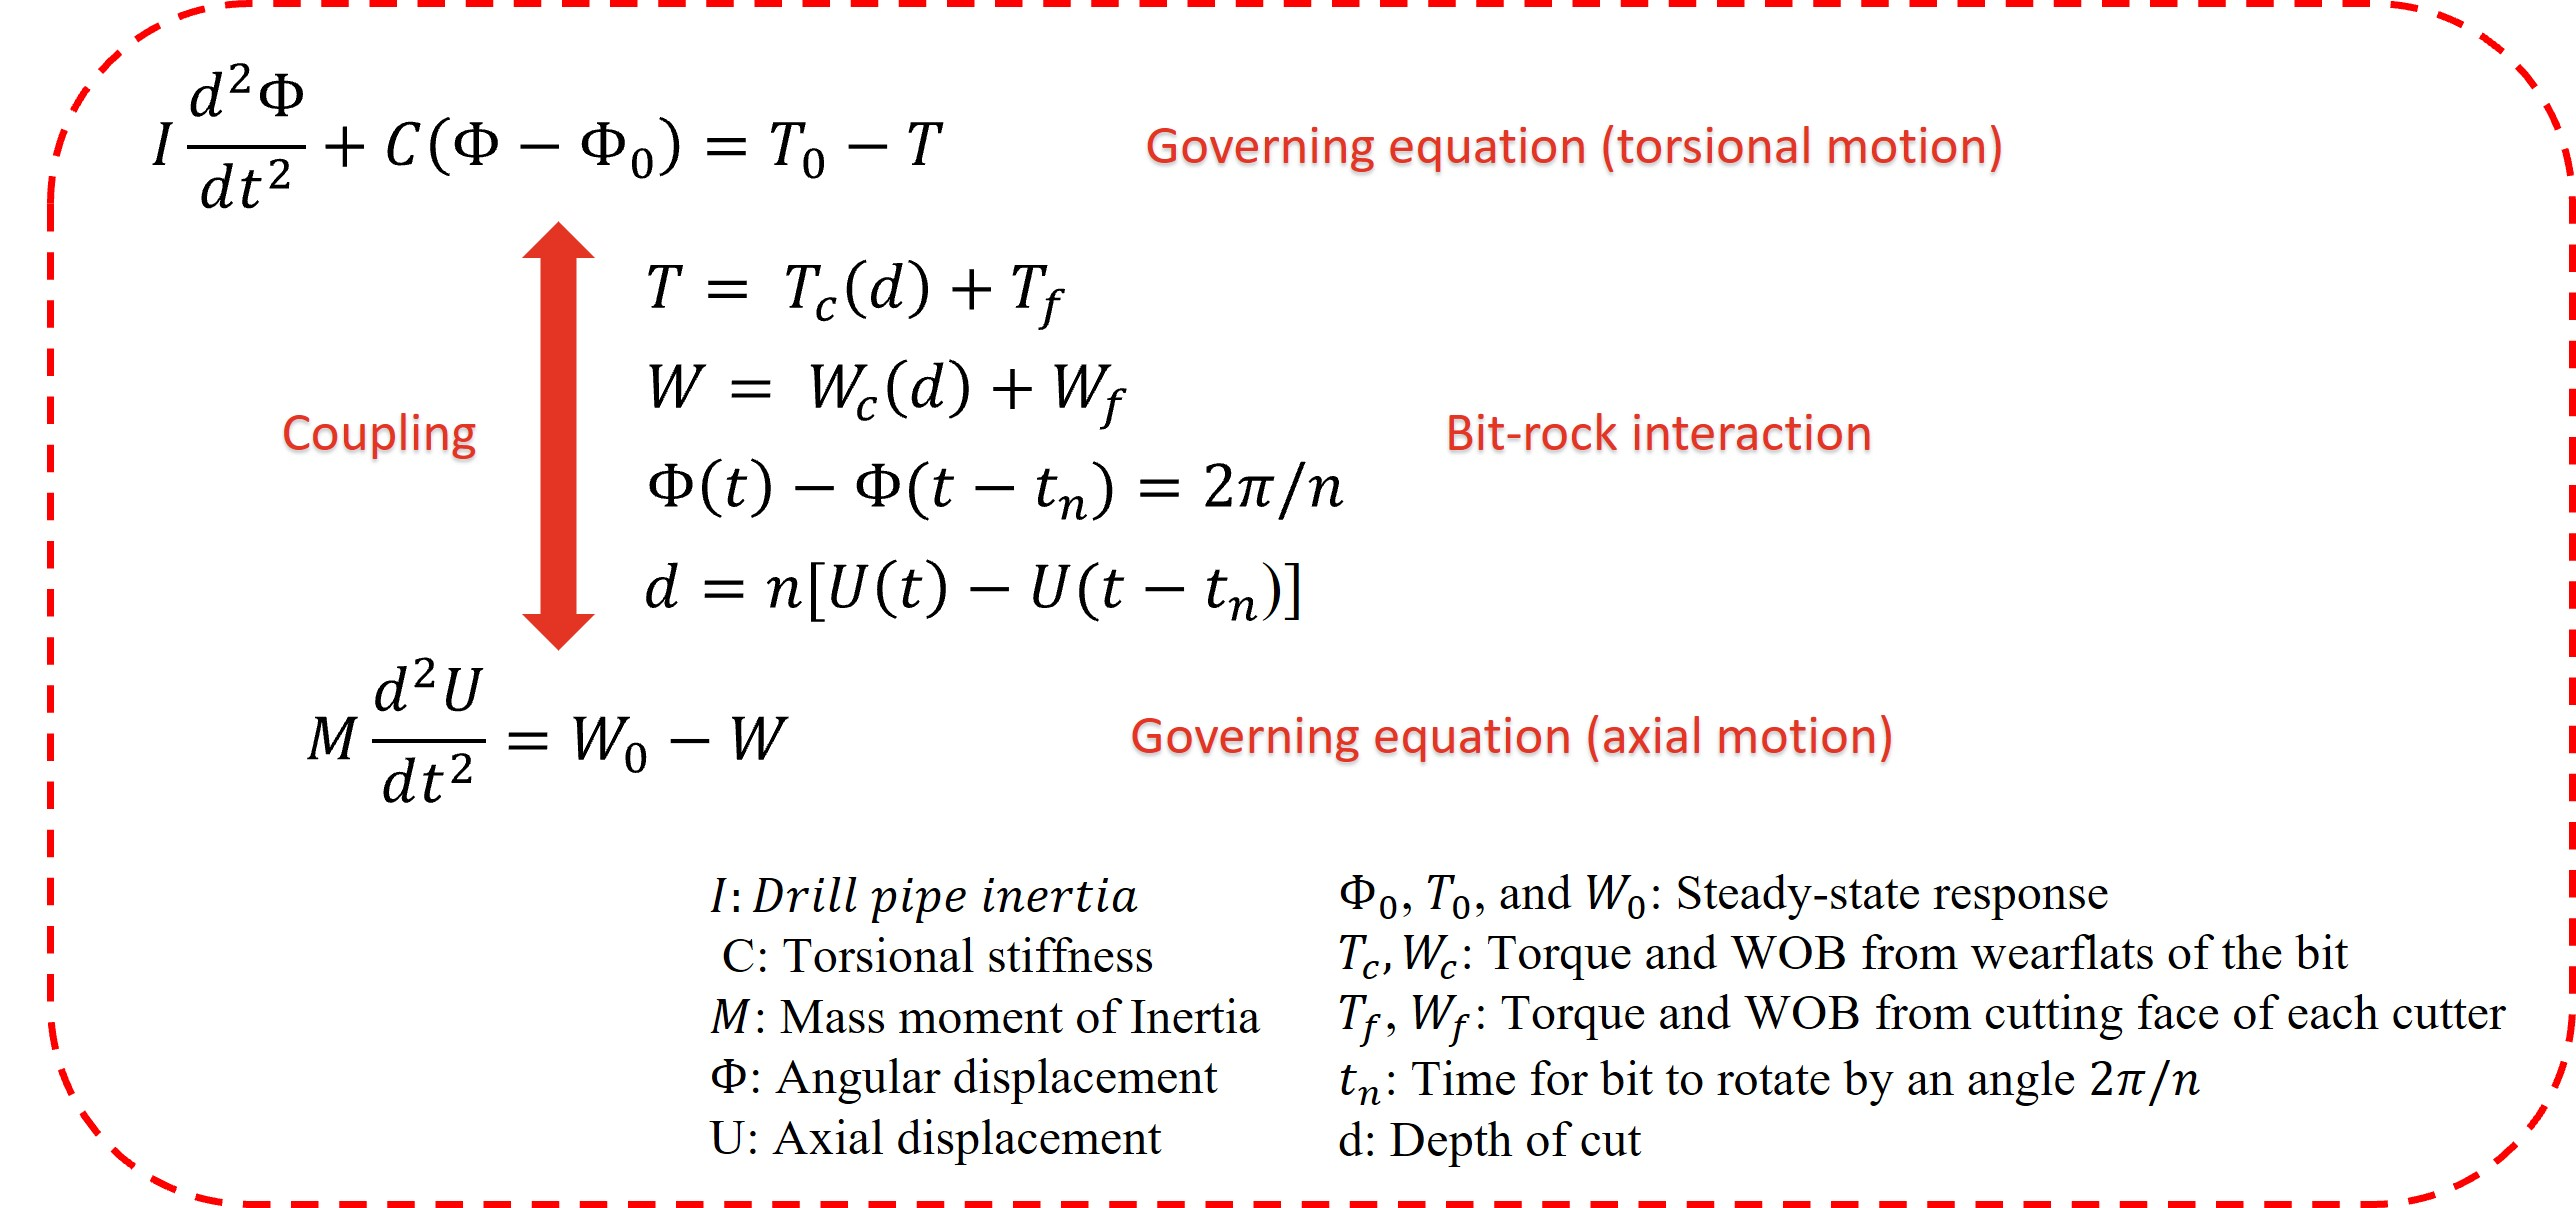
\includegraphics[width=5in]{RGD_summary}
  \caption[Mathematical description of RGD model]{Mathematical description of RGD model.}\label{figure_RGD_Summary}
\end{figure}
\subsection{Extended RGD Model}
Although it was not included in this project, numerous drill string models are benchmarks RGD model for bit-rock interactions, and the model is continuously being developed. \figurename~\ref{model_develop_figure} illustrates the development of the RGD model. Germay increased the degrees of freedom by discretizing the drill string and applying the finite element method \referencename~\cite{ref:germay2009a}. The model was able to model the stick phase occurred by vibration higher than first natural torsional frequency. Similarly, Zhang increased the degrees of the freetom of the model by implementing the spectral method, and further improved the computational efficiency by applying Chebyshev polynomial as a basis funciton \referencename~\cite{ref:zhang2020a}. The model was able to simulate axial and torsional vibrations including stick-slip event with enhanced computationl efficient compared to FEM approach in geometrically simple structure. The source code was not provided so we could not test for this project but these models can be a good candidates for further study. The source code of the RGD model (2 DOF) applying spectral method is provided and mathematical details based on the code can be seen in \appendixname~\ref{ap:rgbworkflow}.

\begin{figure}[ht]
  \centering
  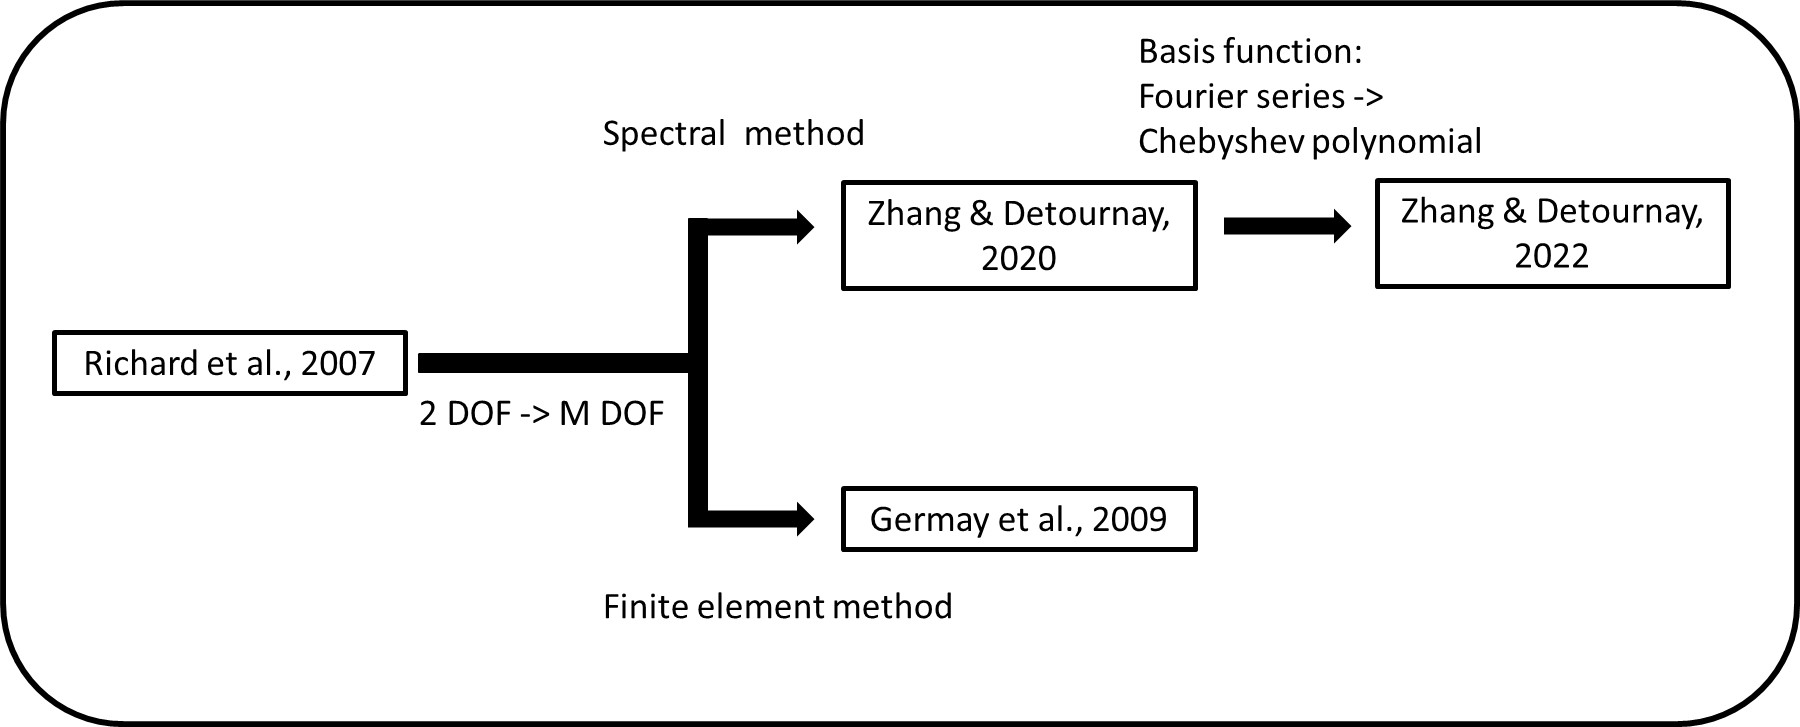
\includegraphics[width=5in]{ModelDevelop}
  \caption[RGD model development]{RGD model development.}\label{model_develop_figure}
\end{figure} 